\thispagestyle{empty}
\subsection{Stack}
\subsubsection*{Recursion Stack (Array version)}
\begin{itemize}
	\item \textbf{Theoretical Time Complexity:} Both implementations have the same theoretical time complexity of O(1) for \verb|push| and O(n) for \verb|copy| operations.
	\item \textbf{Practical Performance:}
	      \begin{itemize}
		      \item  Loop-based implementations are generally faster in practice because they avoid the overhead of function calls and recursion.
		      \item But in the below screenshot, the copy operation with recursive version seems to be faster than the loop version with \(10^{8}\) elements.
		            \begin{figure}[!ht]
			            \centering
			            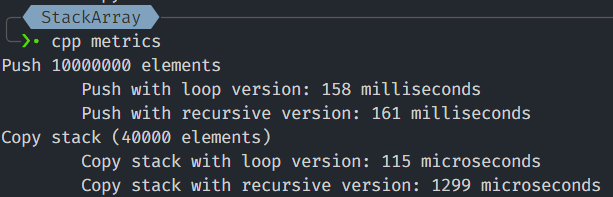
\includegraphics[width=0.6\textwidth]{imgs/StackArray/metrics.png}
			            \caption{Recursive and loop version comparison of Stack (Array version)}\label{fig:stack_arr_metrics}
		            \end{figure}
	      \end{itemize}
\end{itemize}

\subsubsection*{Recursion Stack (Linked List version)}
\begin{itemize}
	\item \textbf{Theoretical Time Complexity:} Both implementations have the same theoretical time complexity of O(1) for \verb|push|, O(n) for \verb|copy| and \verb|release| operations.
	\item \textbf{Practical Performance:}
	      \begin{itemize}
		      \item  Loop-based implementations are generally faster in practice because they avoid the overhead of function calls and recursion.
	      \end{itemize}
\end{itemize}
\begin{figure}[!ht]
	\centering
	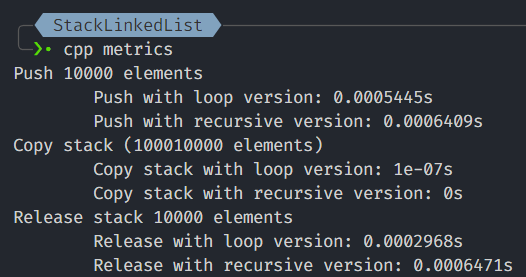
\includegraphics[width=0.6\textwidth]{imgs/StackLinkedList/metrics.png}
	\caption{Recursive and loop version comparison of Stack (Linked List version)}\label{fig:stack_ll_metrics}
\end{figure}